% !TeX root = ../Notizen.tex
\section*{Aufgabe 2: Poincaré Schnitt}
\subsection*{a)}
\begin{figure}[h!]
	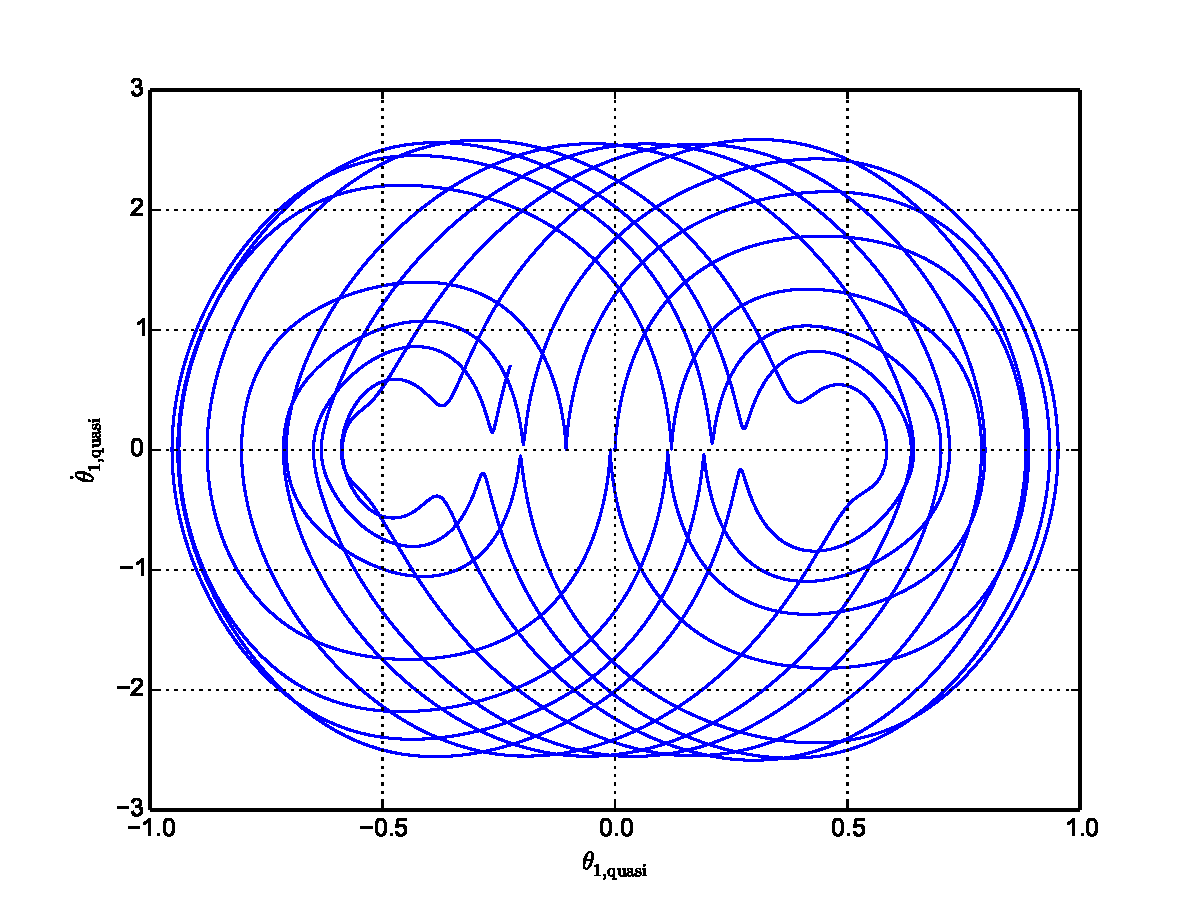
\includegraphics[width = \textwidth]{../Plots/Plot_2_A_1_Phasenraum.pdf}
	\caption{Phasenraum.\label{fig:phasenraum1}}
\end{figure}

\begin{figure}[h!]
	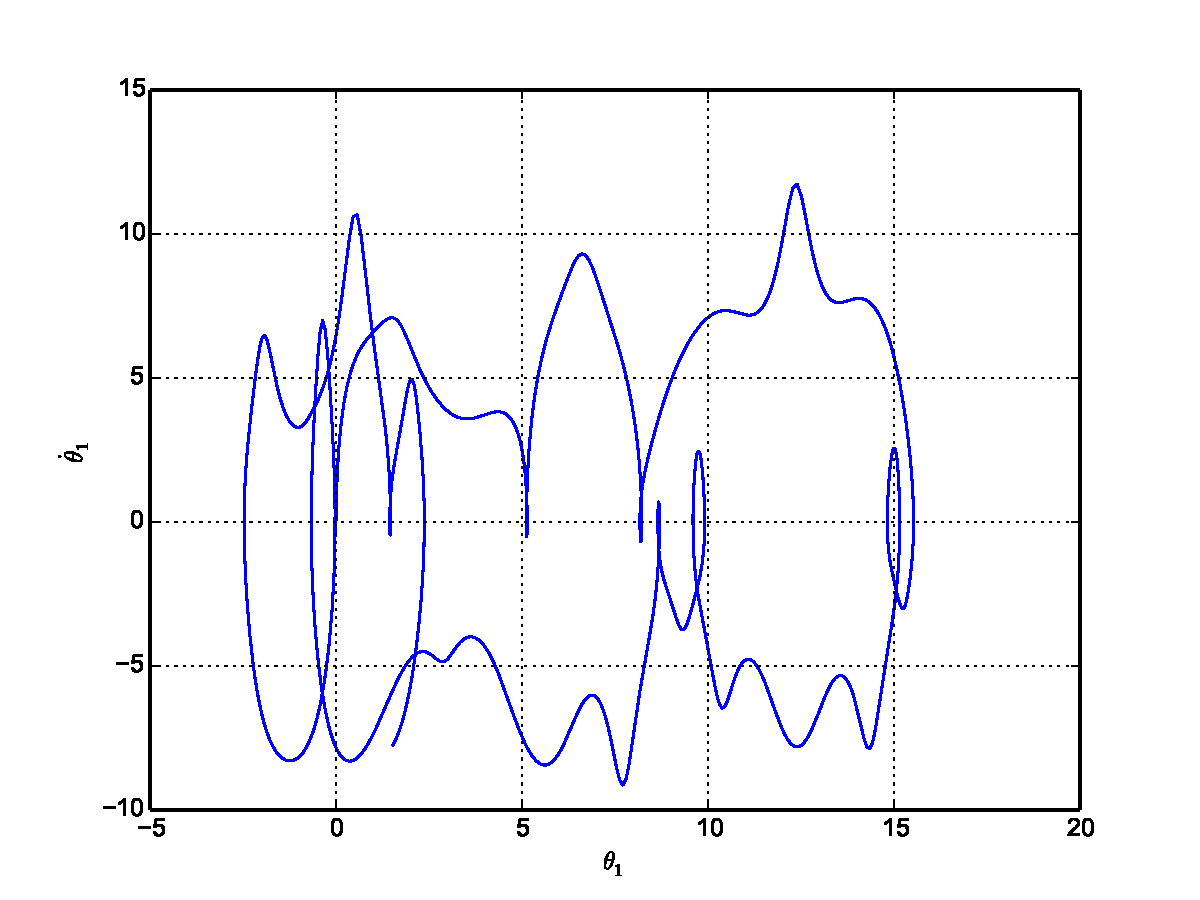
\includegraphics[width = \textwidth]{../Plots/Plot_2_A_2_Phasenraum.pdf}
	\caption{Phasenraum.\label{fig:phasenraum2}}
\end{figure}

\begin{figure}[h!]
	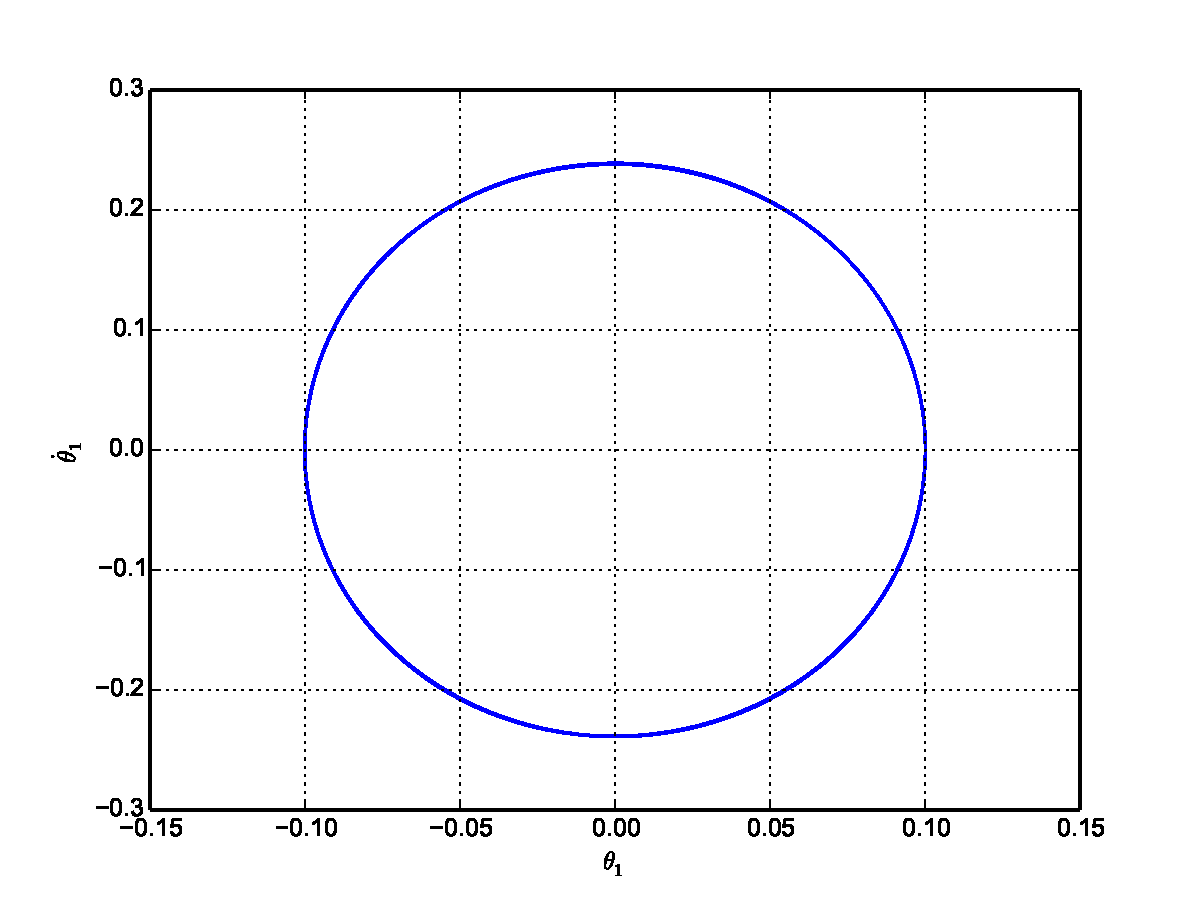
\includegraphics[width = \textwidth]{../Plots/Plot_2_A_3_Phasenraum.pdf}
	\caption{Phasenraum.\label{fig:phasenraum3}}
\end{figure}